\documentclass[journal]{IEEEtran}
\usepackage[a5paper, margin=10mm]{geometry}
%\usepackage{lmodern} % Ensure lmodern is loaded for pdflatex
\usepackage{tfrupee} % Include tfrupee package


\setlength{\headheight}{1cm} % Set the height of the header box
\setlength{\headsep}{0mm}     % Set the distance between the header box and the top of the text


%\usepackage[a5paper, top=10mm, bottom=10mm, left=10mm, right=10mm]{geometry}

%
\setlength{\intextsep}{10pt} % Space between text and floats

\makeindex


\usepackage{cite}
\usepackage{amsmath,amssymb,amsfonts,amsthm}
\usepackage{algorithmic}
\usepackage{graphicx}
\usepackage{textcomp}
\usepackage{xcolor}
\usepackage{txfonts}
\usepackage{listings}
\usepackage{enumitem}
\usepackage{mathtools}
\usepackage{gensymb}
\usepackage{comment}
\usepackage[breaklinks=true]{hyperref}
\usepackage{tkz-euclide} 
\usepackage{listings}
\usepackage{multicol}
\usepackage{xparse}
\usepackage{gvv}
%\def\inputGnumericTable{}                                 
\usepackage[latin1]{inputenc}                                
\usepackage{color}                                            
\usepackage{array}                                            
\usepackage{longtable}                                       
\usepackage{calc}                                             
\usepackage{multirow}                                         
\usepackage{hhline}                                           
\usepackage{ifthen}                                               
\usepackage{lscape}
\usepackage{tabularx}
\usepackage{array}
\usepackage{float}
\usepackage{ar}
\usepackage[version=4]{mhchem}


\newtheorem{theorem}{Theorem}[section]
\newtheorem{problem}{Problem}
\newtheorem{proposition}{Proposition}[section]
\newtheorem{lemma}{Lemma}[section]
\newtheorem{corollary}[theorem]{Corollary}
\newtheorem{example}{Example}[section]
\newtheorem{definition}[problem]{Definition}
\newcommand{\BEQA}{\begin{eqnarray}}
\newcommand{\EEQA}{\end{eqnarray}}

\theoremstyle{remark}


\begin{document}
\bibliographystyle{IEEEtran}
\onecolumn

\title{1.5.15}
\author{INDHIRESH S- EE25BTECH11027}
\maketitle


\renewcommand{\thefigure}{\theenumi}
\renewcommand{\thetable}{\theenumi}

\textbf{Question} The midpoint of the line segment joining $A(2a, 4)$ and $B(-2, 3b)$ is $(1, 2a + 1)$. Findthe values of a and b.\\
\textbf{Solution}:\\
Let us solve the given equation theoretically and then verify the solution computationally. \\
From the given data,
\begin{align}
\vec{A}= \myvec{2a\\4} , \vec{B}=\myvec{-2\\3b}
\end{align}
Let the midpoint of points A and B be C. where,
\begin{align}
    \vec{C}=\myvec{1\\2a+1}
\end{align}
We know that the midpoint formula for the points A and B is
\begin{align}
    \vec{C_x}=\frac{\vec{A_x}+\vec{B_x}}{2}
\end{align}
Where $C_X,A_X\;and\;B_X$ are x coordinates of point C,A and B \\\\
And also A,B and C lies in the same line so they are collinear. So,
\begin{align}
   rank(C-A\;\;\;\;B-A )=1\\
   rank\myvec{1-2a&-2-2a\\
   2a-3&3b-4}=1
\end{align}
From eq.3:
\begin{align}
    \vec{C_x}=\frac{2a-2}{2}
\end{align}
\begin{align}
    1=\frac{2a-2}{2}
\end{align}
\begin{align}
    1=a-1
\end{align}
\begin{align}
    a=2
\end{align}
Now substituiting the value of a in Eq.5, we get:
\begin{align}
     rank\myvec{1-2(2)&-2-2(2)\\
   2(2)-3&3b-4}=1\\
    rank\myvec{-3&-6\\
   1&3b-4}=1
\end{align}
By applying row operation for the matrix\\
$R_2\longrightarrow3R_2+R_1$\\
We get:
\begin{align}
   (C-A\;\;\;\;B-A)=\myvec{-3&-6\\
   0&9b-18}
\end{align}
For the rank to be 1, the second row must be a zero vector. Therefore:
\begin{align}
9b-18=0
\end{align}
\begin{align}
9b=18
\end{align}
\begin{align}
b=2
\end{align}
Therefore the final values of a and b are:
\begin{align}
    a=2\;and\;b=2
\end{align}


From the figure it is clearly verified that the theoretical solution matches with the computational solution.\\
\begin{figure}[h]
    \centering
    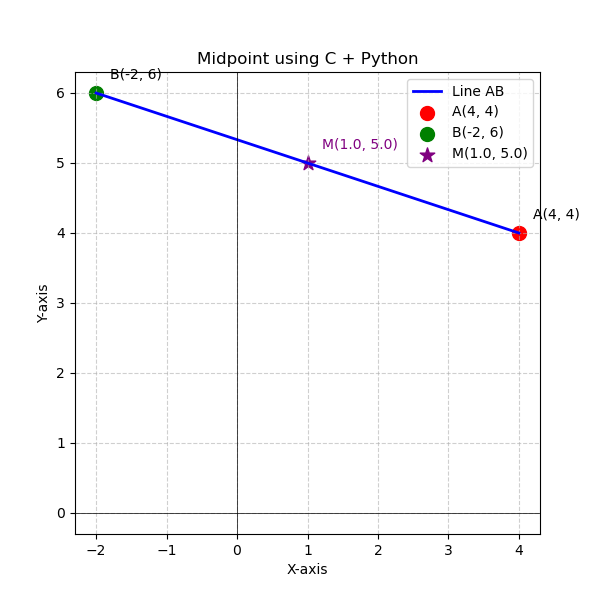
\includegraphics[height=0.5\textheight, keepaspectratio]{figs/figure1.png}
    \label{figure_1}
\end{figure}

\end{document}